\documentclass[12pt, a4paper]{article}
\usepackage[utf8]{inputenc}
\usepackage{pgfplots}
\pgfplotsset{compat=1.18}
\usepackage{geometry}
\geometry{a4paper, margin=2cm}

\begin{document}

\begin{figure}[ht!]
    \centering
    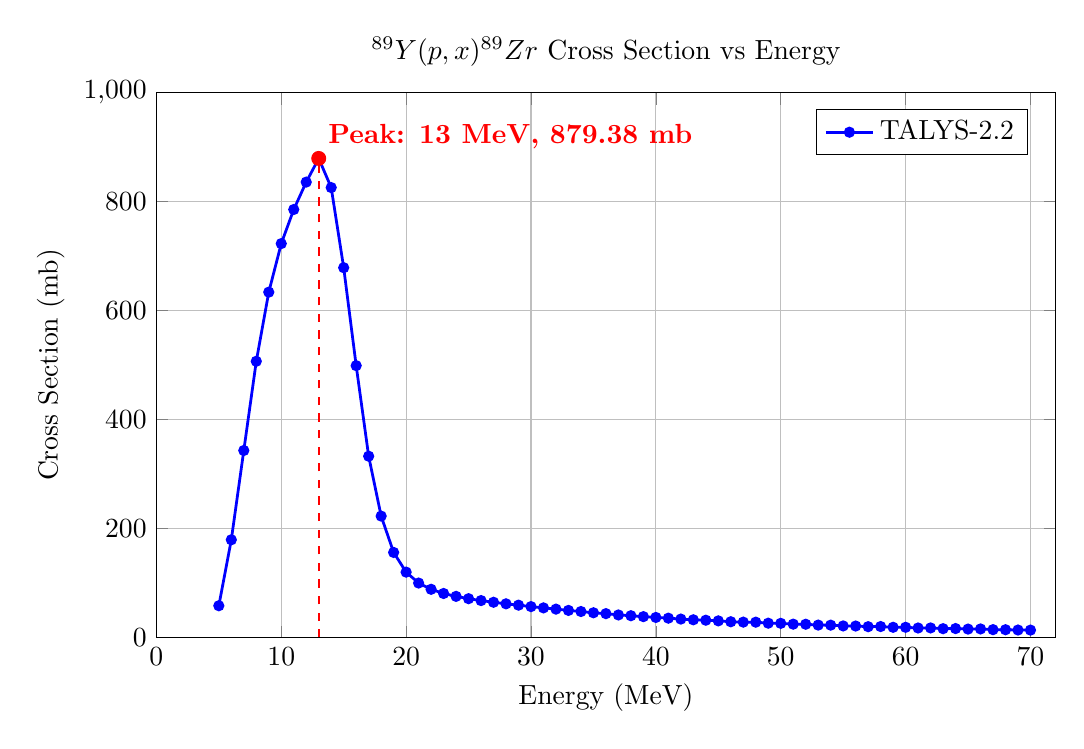
\begin{tikzpicture}
    \begin{axis}[
        title={$^{89}\text{Y}(p,x)^{89}\text{Zr}$ Cross Section vs Energy},
        xlabel={Energy (MeV)},
        ylabel={Cross Section (mb)},
        grid=major,
        width=13cm,
        height=8.5cm,
        xmin=0, xmax=72,
        ymin=0, ymax=1000,
        legend pos=north east
    ]
    
    \addplot[
        color=blue,
        mark=*,
        mark size=1.5pt,
        line width=1pt
    ]
    coordinates {
        (5,58.26)(6,179.34)(7,343.25)(8,507.00)(9,633.91)(10,723.02)
        (11,785.62)(12,835.93)(13,879.38)(14,825.88)(15,678.81)(16,499.01)
        (17,332.75)(18,222.82)(19,156.11)(20,119.98)(21,99.93)(22,88.44)
        (23,80.76)(24,75.47)(25,71.21)(26,67.75)(27,64.65)(28,61.78)
        (29,59.32)(30,56.68)(31,54.33)(32,52.05)(33,49.70)(34,47.67)
        (35,45.37)(36,43.77)(37,41.35)(38,39.97)(39,38.26)(40,36.77)
        (41,35.44)(42,33.79)(43,32.49)(44,31.67)(45,30.50)(46,28.88)
        (47,28.18)(48,28.10)(49,26.25)(50,25.92)(51,24.45)(52,24.29)
        (53,22.76)(54,22.63)(55,21.20)(56,21.02)(57,19.83)(58,20.08)
        (59,18.67)(60,18.69)(61,17.40)(62,17.54)(63,16.15)(64,16.39)
        (65,15.42)(66,15.67)(67,14.39)(68,14.25)(69,13.68)(70,13.54)
    };
    \addlegendentry{TALYS-2.2}
    
    \addplot[mark=*, color=red, mark size=2.5pt] coordinates {(13,879.38)};
    \node[anchor=south west, color=red, font=\bfseries] at (axis cs:13,879.38) {Peak: 13 MeV, 879.38 mb};
    \draw[dashed, red, thick] (axis cs:13,0) -- (axis cs:13,879.38);
    
    \end{axis}
    \end{tikzpicture}
    \caption{$^{89}\text{Y}(p,x)^{89}\text{Zr}$ reaction cross section distribution.}
\end{figure}

\end{document}